\documentclass{article}
\usepackage{graphicx}

\begin{document}
% -----------------------PORTADA-------------------------------------------
\begin{titlepage}
	\centering
	
\includegraphics[width=0.5\textwidth]{unisonlogo.jpg}\par\vspace{1cm}
	{\scshape\LARGE Universidad de Sonora\par}
	\vspace{1cm}
	{\scshape\Large Epigramas de Alan Perlis\par}
	\vspace{1.5cm}
	{\huge\bfseries Lenguajes de Programación\par}
	\vspace{2cm}
	{\Large\itshape Gutierrez Navarro Gustavo\par}
	\vfill
	\vfill
	{\large \today\par}
\end{titlepage}
% -------------------------------------------------------------------------
\begin{center}
    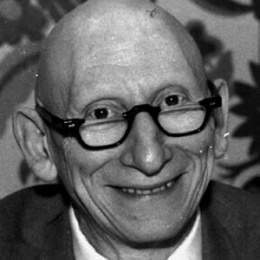
\includegraphics[width=0.5\textwidth]{alan.png}\par\vspace{1cm}
    \huge\textbf{Clasificación de los epigramas de Alan Perlis (sin orden)}
\end{center}
% -------------------------------------------------------------------------
\section{Los diez mejores.}
\begin{itemize}
    % -------------------------------------------------------------------------
    \item[(19)]A language that doesn’t affect the way you think about programming, is not worth knowing.
    \begin{itemize}
        \item Qué significa para ti el epigrama:\\
        Este epigrama describe el objetivo de los distintos de lenguajes de programación. La principal diferencia entre los lenguajes de programación es su manera que tienen de resolver los problemas, por lo tanto, cada uno de estos te obliga a pensar de distinta manera dependiendo del lenguaje que estes usando, por lo tanto, uno que no haga esto no estaría cumpliendo con su objetivo y tendría cero aportaciones a tu conocimiento. Haciendo una analogía, es como tener dos exactamente iguales, pero de distinto color.
        \item Por qué lo elegiste:\\
        Me gusta y comparto esta idea en la que a pesar de que un programa se puede abordar desde distintos lenguajes de programación, cada uno de estos lo resuelve de diferentes formas y es importante conocer el ámbito de tu problema para decidir cuál de todos será más eficiente elegir.
    \end{itemize}
    % -------------------------------------------------------------------------
    % -------------------------------------------------------------------------
    \item[(35)]Everyone can be taught to sculpt: Michelangelo would have had to be taught not to. So it is with great programmers.
    \begin{itemize}
        \item Qué significa para ti el epigrama:\\
        Al momento de intentar enseñar aspectos artísticos de manera sistemática, ocurre en cierta medida una especie de contradicción con la propia naturaleza del arte. El arte debería ser algo creativo y que exprese libertad, sin embargo, al aprenderla de una forma rigurosa y estricta, estas chispas de genialidad se pueden llegar a perder, Alan Perlis propone que algo similar ocurre dentro del campo de la programación. Un factor importante dentro de la computación es la creatividad y en ocasiones se ve reducido debido a las clases en donde se nos educa a escribir código, documentar funciones, pensar soluciones de una única manera, reduciendo nuestra capacidad artística al momento de programar.
        \item Por qué lo elegiste:\\
        Me gusta esta idea por que para mi el programar, quitando formalidades, es únicamente buscar soluciones a problemas y saber traducirlo al lenguaje máquina, por lo tanto gran parte de este trabajo es creativo y creo yo que en muchas ocasiones este mismo se ve atacado por el ambiente computacional actual.
    \end{itemize}
    % -------------------------------------------------------------------------
    % -------------------------------------------------------------------------
    \item[(42)]You can measure a programmer’s perspective by noting his attitude on the continuing vitality of FORTRAN.
    \begin{itemize}
        \item Qué significa para ti el epigrama:\\
        A parte de un sentido mas literal, en donde como programadores debemos intentar ver siempre hacia adelante, no estancándonos en una corriente de pensamiento, un lenguaje, una tecnología o cualquier otro concepto del ambiente. Adicionalmente creo que se puede extrapolar hacia nuestra vida cotidiana. Es importante tener varias perspectivas de la vida, sin embargo, no hay que seguir atados a nuestro pasado.
        \item Por qué lo elegiste:\\
        Tengo dos razones por las cuales me gusto este epigrama. La primera es el mensaje que da y que se explico arriba. El segundo es que se burla de FORTRAN, por lo tanto, se burla de los físicos y eso esta divertido.
    \end{itemize}
    % -------------------------------------------------------------------------
    % -------------------------------------------------------------------------
    \item[(58)]Fools ignore complexity. Pragmatists suffer it. Some can avoid it. Geniuses remove it.
    \begin{itemize}
        \item Qué significa para ti el epigrama:\\
        Uno de los mayores problemas cuando se intenta programar, es la complejidad del algoritmo que se esta desarrollando. Ante esta situación tú, tienes varias formas de enfrentarlo, la más básica seria ni siquiera notar su existencia debido a que no comprendes su dificultad, o tal vez podrías intentar resolverla y sufrir en el intento, también está la opción de intentar buscar otros caminos para rodear esta gran piedra, sin embargo, la mejor opción es removerla, abstraer un problema complejo para hacerlo sencillo. Según Alan Perlis los genios son los encargados de hacer esta última elección, sin embargo, no considero que sea así, todas las personas a pesar de no ser muy dotados intelectualmente podemos tener nuestras chispas de genialidad, lo único que hace falta es dejar de pensar en los problemas de una manera tan sistemática e intentar abordar los problemas de manera mas libre y espontanea, es ahí donde se originan las soluciones realmente increíbles.
        \item Por qué lo elegiste:\\
        Me gusta pensar en esta idea en donde la dificultad del problema la ponemos nosotros. Me he encontrado en situaciones en las que no podía resolver un problema por mas que lo intentara, y sin embargo solo me hacia falta descansar, tomar un respiro y volver a pensar otra vez en el problema, únicamente para darme cuenta que el único que se estaba complicando era yo y no el problema, que en mi desesperado intento por resolverlo nunca me pare a \textbf{pensar}.
    \end{itemize}
    % -------------------------------------------------------------------------
    % -------------------------------------------------------------------------
    \item[(16)]Every program has (at least) two purposes: the one for which it was written, and another for which it wasn’t.
    \begin{itemize}
        \item Qué significa para ti el epigrama:\\
        Para mi en este epigrama se habla un poco del ingenio humano y como una sola herramienta, un solo programa, una sola cosa puede tener hasta varias utilidades. Los ejemplos de estos abundan por toda la historia de la humanidad, desde casos con resultados positivos hasta negativos. Es inevitable que las personas usen tu programa de manera indebidas, sin embargo, no es algo malo per se, incluso se podría decir que es algo natural del ser humano.
        \item Por qué lo elegiste:\\
        Esta interesante esta idea que todos los programas (salvando distancias con los programas muy básicos) pueden ser utilizados de distintas maneras, incluso usar estos programas para crear otros.
    \end{itemize}
    % -------------------------------------------------------------------------
    % -------------------------------------------------------------------------
    \item[(66)]Making something variable is easy. Controlling duration of constancy is the trick.
    \begin{itemize}
        \item Qué significa para ti el epigrama:\\
        Yo entiendo esta frase de dos maneras. La primera se refiere a la vida, en donde dejar que las cosas varíen y cambien durante el tiempo es fácil pero lo complicado es mantener algo constante por cierto tiempo, ya sea un pensamiento, una idea o una rutina. Por otro lado, en programación entiendo el concepto de constancia como dejar un valor igual por el transcurso de un tiempo y que en ocasiones, algunas funciones o procesos de las que no tenemos el control total modifican estos valores que no se quieren cambiar, por lo tanto, el controlar estos pequeños detalles esconde el secreto de ser un buen programador.
        \item Por qué lo elegiste:\\
        Esta muy interesante este detalle de no hablar de la constancia como algo invariable, si no mas bien una especie de subconjunto de las variables. Es similar a tomar los dos extremos de las posturas y escoger el punto medio de estas, una constante que varía con el tiempo. Me gusta esta idea porque creo que es un razonamiento muy sano que se puede aplicar a nuestras vidas.
    \end{itemize}
    % -------------------------------------------------------------------------
    % -------------------------------------------------------------------------
    \item[(7)]It is easier to write an incorrect program than understand a correct one.
    \begin{itemize}
        \item Qué significa para ti el epigrama:\\
        En términos literales, el escribir un código incorrecto es mucho mas probable que escribir uno correcto, incluso puedes lograr escribir un código de manera efectiva y aun así no entenderlo. La palabra entender dentro del mundo de la computación es una palabra muy fuerte, realmente hay muy pocos conceptos que llegas a entender en su totalidad, claro que puedes comprender hasta cierta parte, pero su completitud esta muy alejada del alcance de muchos.
        \item Por qué lo elegiste:\\
        Lo elegí, porque de cierta forma me hace darme cuenta de las tantas cosas que realmente no entiendo a pesar de hacerlas.
    \end{itemize}
    % -------------------------------------------------------------------------
    % -------------------------------------------------------------------------
    \item[(20)]Wherever there is modularity there is the potential for misunderstanding: Hiding information implies a need to check communication.
    \begin{itemize}
        \item Qué significa para ti el epigrama:\\
        Extrapolando todo el concepto de la programación orientada a objetos y aplicándolo la vida cotidiana, podemos observar este caso en las redes de comunicación que en algún punto pueden llegar a corromperse, lo que se conoce como el teléfono descompuesto o los malentendidos ocasionados por mentiras, esto ocurre tanto en la vida como en la computación.
        \item Por qué lo elegiste:\\
        Me gusto por que he tenido varias experiencias respecto a la mala comunicación que han llevado a situaciones desfavorables. Además, soy una persona que considera el hablar como la única manera de resolver los problemas.
    \end{itemize}
    % -------------------------------------------------------------------------
    % -------------------------------------------------------------------------
    \item[(39)]Re graphics: A picture is worth 10K words - but only those to describe the picture. Hardly any sets of 10K words can be adequately described with pictures.
    \begin{itemize}
        \item Qué significa para ti el epigrama:\\
        Citando el viejo dicho de: “Una imagen dice mas que mil palabras”. Analizando esta frase desde dos puntos de vista, desde el computacional podemos enfocarlo desde la visión de bits, en donde una sola imagen no es más que un conjunto inmenso de pixeles que se unen para formar una imagen. El otro punto de vista, mas alejado del a computación es el pensar como una solo una imagen puede transmitir tanto, en cuanto tu cerebro observa una foto, de manera automática empieza el análisis de esta, los colores, la composición, el significado detrás del cuadro, las metáforas, su simbolismo y un sinfín más, en cambio a nuestro cerebro le cuesta mas crear una imagen a partir de conceptos o ideas que le demos.
        \item Por qué lo elegiste:\\
        Lo elegí porque noté el gran cambio respecto a la época en donde se escribió estos epigramas. Para la gran sorpresa de muchos, actualmente se pueden generar imágenes a partir de varias palabras, todavía se siguen alejando de la cifra propuesta por Perlis, pero al menos es una avance.
    \end{itemize}
    % -------------------------------------------------------------------------
    % -------------------------------------------------------------------------
    \item[(95)]Don’t have good ideas if you aren't willing to be responsible for them.
    \begin{itemize}
        \item Qué significa para ti el epigrama:\\
        Una de las virtudes mas grandes que tiene la computación es la gran capacidad de creación que posee, la gran mayoría de cosas que se imagine una persona, se pueden realizar en la computadora. Si estas dispuesto a pensar grandes ideas, también debes tener la responsabilidad de llevarlas a cabo y no renunciar a ellas por simples excusas.
        \item Por qué lo elegiste:\\
        Me gusta esta idea por que de cierta forma me motiva, a dejar de pensar cosas que me gustaría hacer y ponerme a hacerlas. Hace años cuando iba en preparatoria, soñaba con crear un programa capaz de imitar la voz de una persona, ahora me doy cuenta que posiblemente no hice caso al epigrama.
    \end{itemize}
    % -------------------------------------------------------------------------
\end{itemize}
% -------------------------------------------------------------------------
\section{Los diez peores}
\begin{itemize}
    % -------------------------------------------------------------------------
    \item[(27)]Once you understand how to write a program get someone else to write it.
    \begin{itemize}
        \item Qué significa para ti el epigrama:\\
        Este programa lo asemejo bastante a lo que ocurre en el sistema laboral en el área de computación. La jerarquía social y laboral que existe entre el junior y senior, donde este último (que previamente ya paso por todo el proceso del primero) es el encargado de dirigir a los pequeños. Puede ser que en la época de Alan Perlis este concepto no estuviera tan deteriorado, pero actualmente ocurre bastante que las personas que apenas están entrando en el mundo laboral apenas y tienen oportunidad de realizar innovaciones o generar sus propias soluciones, es muy común que el proceso creativo lo desarrolle el senior, mientras que el otro únicamente se encarga de recibir y actuar.
        \item Por qué lo elegiste:\\
        No me gusta el mensaje que se da en el que el senior tiene una superioridad intrínseca únicamente por el puesto que ostenta, es cierto que en el gran mayor de los casos debido a su experiencias ellos son los que tienen la razón, sin embargo, no creo que únicamente por su rol este en lo correcto de manera automática.
    \end{itemize}
    % -------------------------------------------------------------------------
    % -------------------------------------------------------------------------
    \item[(85)]Though the Chinese should adore APL, it’s FORTRAN they put their money on.
    \begin{itemize}
        \item Qué significa para ti el epigrama:\\
        Considerando el hecho que tal vez no entienda del todo este epigrama, según mi punto de vista es simplemente que los chinos desarrollan FORTRAN a pesar de la creencia popular que dice que usan APL.
        \item Por qué lo elegiste:
        Es bastante simple, algo racista y sin gracia.
    \end{itemize}
    % -------------------------------------------------------------------------
    % -------------------------------------------------------------------------
    \item[(79)]A year spent in artificial intelligence is enough to make one believe in God.
    \begin{itemize}
        \item Qué significa para ti el epigrama:\\
        El epigrama hace una pequeña broma en la que aprender sobre inteligencia artificial es complicado, que incluso te hace llegar a creer en dios.
        \item Por qué lo elegiste:\\
        No me gusta porque es un chiste bastante básico, y pues realmente no se me hace muy interesante más allá del chistecito (que ni me da risa).
    \end{itemize}
    % -------------------------------------------------------------------------
    % -------------------------------------------------------------------------
    \item[(93)]When someone says ”I want a programming language in which I need only say what I wish done,” give him a lollipop.
    \begin{itemize}
        \item Qué significa para ti el epigrama:\\
        La programación es una disciplina la cual se necesita pensar y razonar, por lo tanto, si no estás dispuesto a ello, entonces deberías dedicarte a otra cosa.
        \item Por qué lo elegiste:\\
        Realmente no me desagrada, pero tampoco me agrada, me es indiferente este epigrama.
    \end{itemize}
    % -------------------------------------------------------------------------
    % -------------------------------------------------------------------------
    \item[(40)]There are two ways to write error-free programs; only the third one works.
    \begin{itemize}
        \item Qué significa para ti el epigrama:\\
        El significado detrás de esta frase es simple, no existe una manera de construir un programa sin errores.
        \item Por qué lo elegiste:\\
        A pesar de compartir el significado del epigrama, se me hace bastante simple y básico.
    \end{itemize}
    % -------------------------------------------------------------------------
    % -------------------------------------------------------------------------
    \item[(61)]In programming, as in everything else, to be in error is to be reborn.
    \begin{itemize}
        \item Qué significa para ti el epigrama:\\
        El cometer un error forma parte del proceso de aprendizaje, después del error no te garantiza el no volver a equivocarte ni tampoco el lograr tu objetivo, sin embargo, en ocasiones el camino hacia una meta resulta tener mas valor que la propia meta.
        \item Por qué lo elegiste:\\
        Creo que es un concepto bastante quemado, el equivocarte para aprender y luego lograr tus objetivos y posiblemente por eso no me gusto.
    \end{itemize}
    % -------------------------------------------------------------------------
    % -------------------------------------------------------------------------
    \item[(63)]When we write programs that ”learn”, it turns out that we do and they don’t.
    \begin{itemize}
        \item Qué significa para ti el epigrama:\\
        Para mi significa que cuando intentamos escribir programas que aprenden, como lo podrían los de inteligencia artificial, al final resulta que los que aprendimos algo fuimos nosotros (refiriéndose a los conocimientos teóricos y prácticos obtenidos) y que la maquina no lo hizo. También se puede aplicar cuando estamos explicando un concepto a alguien, al final resulta que esa explicación nos ayudó a nosotros a reforzar ciertos conocimientos mientras que la otra persona realmente no entendió.
        \item Por qué lo elegiste:\\
        Viendo esta frase en retrospectiva, realmente no queda muy bien ya que actualmente la inteligencia artificial es una realidad.
    \end{itemize}
    % -------------------------------------------------------------------------
    % -------------------------------------------------------------------------
    \item[(65)]Make no mistake about it: Computers process numbers - not symbols. We measure our
understanding (and control) by the extent to which we can arithmetize an activity.
    \begin{itemize}
        \item Qué significa para ti el epigrama:\\
        Al final de todo, si nos ponemos a pensar detalladamente, cualquier cosa que se haga en la computadora, no es mas que el resultado de operaciones aritméticas, por lo tanto, hasta ese punto llega nuestro control.
        \item Por qué lo elegiste:\\
        No comparto este pensamiento, a pesar de ser cierto considero que una gran parte del avance que existe en la computación se debe al enfoque desde varias perspectivas de la computación y limitarse a ver a las computadoras como maquinas de operaciones entre binarios resultara en una limitación de la tecnología.
    \end{itemize}
    % -------------------------------------------------------------------------
    % -------------------------------------------------------------------------
    \item[(76)]It is the user who should parameterize procedures, not their creators.
    \begin{itemize}
        \item Qué significa para ti el epigrama:\\
        Entiendo esta frase como que, al momento de realizar funciones para los usuarios, los encargados de decidir qué información necesitan estas funciones son ellos mismos y no el programador, la razón se debe a que finalmente el que usara estas funciones son ellos y no los creadores.
        \item Por qué lo elegiste:\\
        A pesar de compartir ciertas ideas en este punto, considero que no es del todo cierto y que finalmente la responsabilidad recae en el programador, es importante escuchar la opinión del cliente mas no dejar que el ponga los precios del restaurante.
    \end{itemize}
    % -------------------------------------------------------------------------
    % -------------------------------------------------------------------------
    \item[(3)]Syntactic sugar causes cancer of the semicolon.
    \begin{itemize}
        \item Qué significa para ti el epigrama:\\
        Referente a la sintaxis de un escrito. El azúcar vendría a ser las reglas que tiene el mismo, y si durante la creación de estas se abusa de ellas, se llega a un elemento que no es necesario en los lenguajes de programación, lo que vendría a ser el cáncer de colon, haciendo un juego de palabras con el punto y coma.
        \item Por qué lo elegiste:\\
        Esta medio malo el chiste la verdad, y pues no da risa.
    \end{itemize}
    % -------------------------------------------------------------------------
\end{itemize}
% -------------------------------------------------------------------------
\end{document}